
%----------------------------------------------------------------------------------------
%	PACKAGES AND OTHER DOCUMENT CONFIGURATIONS
%----------------------------------------------------------------------------------------

\documentclass[12pt]{article} % Default font size is 12pt, it can be changed here

\usepackage{geometry} % Required to change the page size to A4
\geometry{a4paper} % Set the page size to be A4 as opposed to the default US Letter

\usepackage{graphicx} % Required for including pictures

\usepackage{float} % Allows putting an [H] in \begin{figure} to specify the exact location of the figure


\linespread{1.2} % Line spacing

%\setlength\parindent{0pt} % Uncomment to remove all indentation from paragraphs

\graphicspath{{Pictures/}} % Specifies the directory where pictures are stored

\begin{document}

%----------------------------------------------------------------------------------------
%	TITLE PAGE
%----------------------------------------------------------------------------------------

\begin{titlepage}

\newcommand{\HRule}{\rule{\linewidth}{0.5mm}} % Defines a new command for the horizontal lines, change thickness here

\center % Center everything on the page

\textsc{\LARGE Enseeiht}\\[1.5cm] % Name of your university/college
\textsc{\Large Projet Long}\\[0.5cm] % Major heading such as course name
\textsc{\large M�thodes de clustering parall�les}\\[0.5cm] % Minor heading such as course title

\HRule \\[0.4cm]
{ \huge \bfseries Test Plan}\\[0.4cm] % Title of your document
\HRule \\[1.5cm]

\begin{minipage}{0.4\textwidth}
\begin{flushleft} \large
\emph{Project Manager:}\\
Tristan \textsc{Soriano} % Your name
\end{flushleft}
\end{minipage}
~
\begin{minipage}{0.4\textwidth}
\begin{flushright} \large
\emph{Supervisor:} \\
Laurent \textsc{Beugnet} % Supervisor's Name
\end{flushright}
\end{minipage}\\[4cm]

\begin{minipage}{0.4\textwidth}
\begin{flushleft} \large
\emph{Client IRIT:}\\
Ronan \textsc{Guivarch} % Your name
Sandrine \textsc{Mouysset}
\end{flushleft}
\end{minipage}




%{\large \today}\\[3cm] % Date, change the \today to a set date if you want to be precise

%\includegraphics{Logo}\\[1cm] % Include a department/university logo - this will require the graphicx package

\vfill % Fill the rest of the page with whitespace

\begin{figure}[H] % Example image
\center{
\includegraphics[width=0.5\linewidth]{INP-n7.png}}

\end{figure}

\end{titlepage}

%----------------------------------------------------------------------------------------
%	TABLE OF CONTENTS
%----------------------------------------------------------------------------------------

\tableofcontents % Include a table of contents

\newpage % Begins the essay on a new page instead of on the same page as the table of contents 
%-----------------------------------------------------------------------------------------


\section{Presentation}

\subsection{Name} % Sub-section
New clustering methods integration into a parallel code.
\subsection{Sponsort}
IRIT : Ronan Guivarch, Sandrine Mouysset.
\subsection{Presentation}
The purpose of the project is to add new clustering methods into an existing piece of software. The clustering method are used on dense and sparse matrix which involve heavy computing calculus and time processing. In order to solve such issue, the existing code run on a master slave architecture. The original image is splitted among different slaves that compute initially a single clustering method: spectral clustering. 
\begin{figure}[H] % Example image
\center{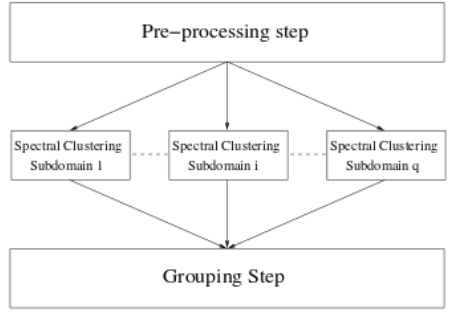
\includegraphics[width=0.5\linewidth]{masterslave.png}}
\caption{}
\label{fig:speciation}
\end{figure}
The objective is first to add two methods : Kernel K-means and Mean shift in such structure then to refactore/clean the existing code.

\section{Environment}
\subsection{Hardware environment}
As it is a parallel computing program. The environment must enable the team to test on single and on multiple entity the code produced. In order to do so the code will be tested on lab machines, which are the most likely to represent the IRIT environment. 
\subsection{Software environment}
This project implies the use of multiple technologies: Matlab, Fortran, MPI, ssh, Doxygen. The test must run on the client machine configuration.

\section{Test definition}
The following test must show the client that the code fit the specifications. It include non-regression test : the original code will be tested on the team configuration as a performance reference and will be compared to the new implemented algorithm result in term of efficiency and quality.

\textbf{Id}: T001
\textbf{Description}: This is the initial test, all the initial function of the program must run. \\
bouquet, 3blocSimples, Cible, arthus will be tested\\
\textbf{Result} : The program must run on 2D, 3D geometrical and color images. \\
Bouquet: It must produce 4 clusters : leaf, oranges, tree, backgroung.\\
Cible: It must produce 1 cluster per ring.\\
3blocSimples: 3 clusters\\
Arthus: It must run, find clusters in a limited time.\\

\textbf{Id}: T002
\textbf{Description}: We must test the matlab implmentation of Mean Shift \\
bouquet, 3blocSimples, Cible will be tested\\
\textbf{Result}: The program must run on 2D, 3D geometrical and color images. \\
Bouquet: It must produce 4 clusters : leaf, oranges, tree, backgroung.\\
3blocSimples: 3 clusters\\
Cible: It must produce 1 cluster per ring.\\

\textbf{Id}: T003
\textbf{Description}: We must test the matlab implmentation of Kernel K-Means \\
bouquet, 3blocSimples, Cible will be tested\\
\textbf{Result}: The program must run on 2D, 3D geometrical and color images. \\
Bouquet: It must produce 4 clusters : leaf, oranges, tree, backgroung.\\
Cible: It must produce 1 cluster per ring.\\
3blocSimples: 3 clusters\\

\textbf{Id}: T004
\textbf{Description}: We must test the Fortran implmentation of Mean Shift \\
bouquet, 3blocSimples, Cible will be tested\\
\textbf{Result}: The program must run on 2D, 3D geometrical and color images. \\
Bouquet: It must produce 4 clusters : leaf, oranges, tree, backgroung.\\
Cible: It must produce 1 cluster per ring.\\
3blocSimples: 3 clusters\\

\textbf{Id}: T005
\textbf{Description}: We must test the Fortran implmentation of Mean Shift \\
Arthus1 will be tested with different bandwidth\\
\textbf{Result}: The program must run on 2D, 3D geometrical and color images. \\
Arthus 1 must produce an image segmentation result in limited time\\

\textbf{Id}: T006
\textbf{Description}: We must test the Fortran implmentation of Kernel K-means \\
bouquet, 3blocSimples, Cible will be tested: 
\begin{enumerate}
\item using polynomial kernel function
\item using gaussian kernel function
\end{enumerate}
\textbf{Result}: The program must run on 2D, 3D geometrical and color images. \\
Bouquet: It must produce 4 clusters : leaf, oranges, tree, backgroung.\\
Cible: It must produce 1 cluster per ring.\\
3blocSimples: 3 clusters\\

\textbf{Id}: T007
\textbf{Description}: We must test the initial implmentation of Spectral clustering using different Kernel function \\
bouquet, 3blocSimples, Cible will be tested: 
\begin{enumerate}
\item using polynomial kernel function
\item using gaussian kernel function
\end{enumerate}
\textbf{Result}: The program must run on 2D, 3D geometrical and color images. \\
Bouquet: It must produce 4 clusters : leaf, oranges, tree, backgroung.\\
Cible: It must produce 1 cluster per ring.\\
3blocSimples: 3 clusters\\

The test T005 o T007 will be duplicated for parallel computing

Thoose test will cover:
\begin{enumerate}
\item Matlab implementation of Kernek K-means
\item Matlab implementation of Mean shift
\item Fortran implementation of Kernek K-means
\item Fortran implementation of Mean shift
\item Fortran implementation of Kernel methods
\item Integration of the methods into a parallel code
\end{enumerate}


\textbf{Id}: T008
\textbf{Description}: We must show that the code refactoring has een succesull \\
The code will e satical analysed to show the improvement 

\textbf{Result}: The code readability, syntax must have been improved and standards must have applied : one language, one naming standard etc\\

\end{document}



